\section{Parallel histogram calculation using OpenMP \punkte{15}}

To explore different synchronization strategies in OpenMP, I implemented three parallel versions of the histogram computation: 
an \texttt{atomic} version, a \texttt{Merge Critical} version (where the merge occurs inside the parallel region), 
and a \texttt{Merge Out} version (where the merge is done sequentially outside).  
The goal was to understand how the placement of synchronization and merging affects performance and scalability.

\subsection*{Implementation}
All implementations were based on the same sequential structure but used different OpenMP synchronization mechanisms.  
Listings~\ref{lst:mergeCritical}, \ref{lst:mergeOut}, and \ref{lst:atomic} show the relevant code excerpts, pulled directly from \texttt{Skeleton\_codes/hist/hist\_omp.cpp}.

\lstinputlisting[
    language=C++,
    numbers=left,
    caption={Histogram with private histograms and in-region merge (Merge Critical)},
    captionpos=b,
    label={lst:mergeCritical},
    linerange={38-59},
    firstnumber=38
]{../Skeleton_codes/hist/hist_omp.cpp}

\lstinputlisting[
    language=C++,
    numbers=left,
    caption={Histogram with private histograms and external merge (Merge Out)},
    captionpos=b,
    label={lst:mergeOut},
    linerange={61-89},
    firstnumber=61
]{../Skeleton_codes/hist/hist_omp.cpp}

\lstinputlisting[
    language=C++,
    numbers=left,
    caption={Histogram with atomic updates},
    captionpos=b,
    label={lst:atomic},
    linerange={91-99},
    firstnumber=91
]{../Skeleton_codes/hist/hist_omp.cpp}

The \texttt{Merge Critical} version was designed with the idea that a thread finishing early could immediately start merging its partial results,
while the others were still computing.  
Conversely, in the \texttt{Merge Out} version, all threads first complete the heavy computation before performing a single sequential merge.

\subsection*{Performance analysis}
Figure~\ref{fig:histScaling} (\textit{placeholder path to be updated}) reports the strong scaling results obtained on the cluster.  
Up to the number of available physical cores (around 16–20), both versions scale well, but the \texttt{Merge Out} version performs slightly better overall.
This suggests that avoiding synchronization inside the parallel region provides better efficiency, despite the merge being fully sequential at the end.  
The expected advantage of the in-region merge (starting earlier) was not visible in practice, likely because the cost of locking and cache contention outweighed the benefit.

It is interesting to note that for the \texttt{Merge Critical} version, increasing the number of threads from 8 to 16 actually worsens the runtime, which is counterintuitive 20 cores were available. This behavior is probably related to increased contention on the critical section lock and the underlying OpenMP runtime scheduling and synchronization overheads.

It is also noteworthy that the \texttt{atomic} version performed poorly at all thread counts, even worse than the sequential baseline.  
This is due to high contention and cache-line conflicts, as each atomic increment effectively serializes access to the shared histogram array.

\begin{figure}[H]
    \centering
    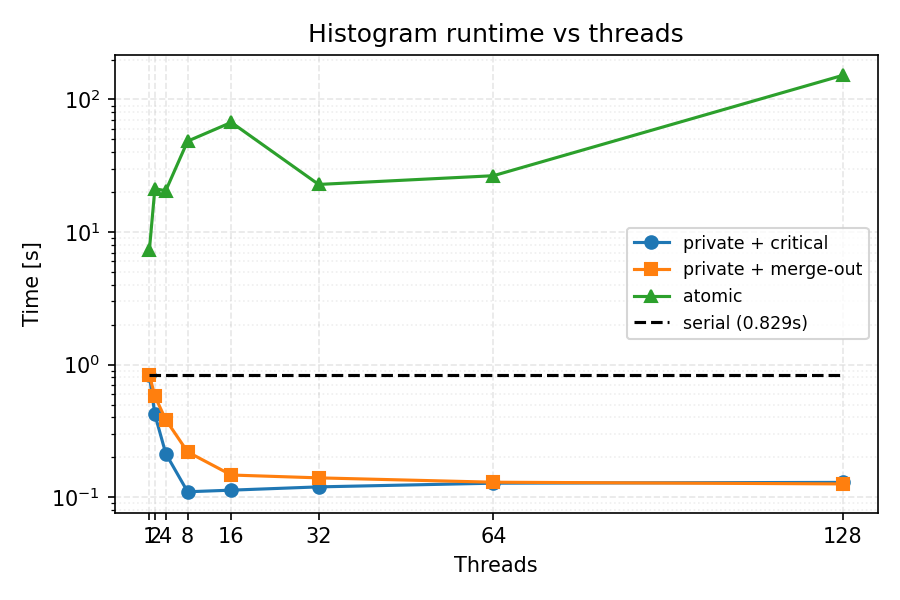
\includegraphics[width=0.8\textwidth]{../Skeleton_codes/hist/plots/hist_runtime_scaling.png}
    \caption{Strong scaling of the three OpenMP histogram versions.}
    \label{fig:histScaling}
\end{figure}

\noindent
In summary, the results show that minimizing synchronization inside the parallel section is key for performance.
While both merge strategies are correct, the external merge (\texttt{Merge Out}) achieves better scalability,
and the atomic approach is clearly inefficient for this workload.
